\chapter{Planning Algorithm}
\label{planning_algo}
\section{Introduction}

The goal of the path planner is to navigate the robot from the start state to destination by blending in the traffic. Path planning module is dependent on various modules to receive the data regarding the perceived environment and invoke a set of modules to move the ego vehicle safely. It has to drive the ego vehicle forward considering the traffic rules, obstacles, kinematic and dynamic constraints of the robot and not compromising on the safety and comfort of the passengers inside. This chapter aims to describe path planning techniques developed in this thesis to drive the ego vehicle safely to the destination.

This section is organised to provide an overview of different modules needed for path planning and methods used in each module to achieve the goal. Path planning starts from the initial understanding of where the ego vehicle is and where to go, subsection \ref{localization} describes the localisation of ego vehicle to provide this data, subsection \ref{route_planner} provides the information on how a global path to the destination is calculated. An autonomous vehicle should have an understanding of surroundings concerning where other vehicles are, where pedestrians are, traffic signal information etc. Prediction module described in \ref{prediction} details further on how the ego vehicle perceives the environment. The next subsection \ref{motion_planner} describes in-depth details on the short-term planning algorithm aka trajectory planner. The final module in the discussion is control unit, described in subsection \ref{traj_follower}. It is responsible for translating the path in space-time into steering and acceleration values to drive the ego vehicle.

Figure \ref{path_planner} represents the general architecture of the planning module. It details on the flow of information, dependencies, relative execution frequency. The components in dark blue are the primary focus of this thesis, parts in light blue are adopted from other works and modules in sky blue are preexisting or simulated. 
\begin{figure}[h]
    \centering
    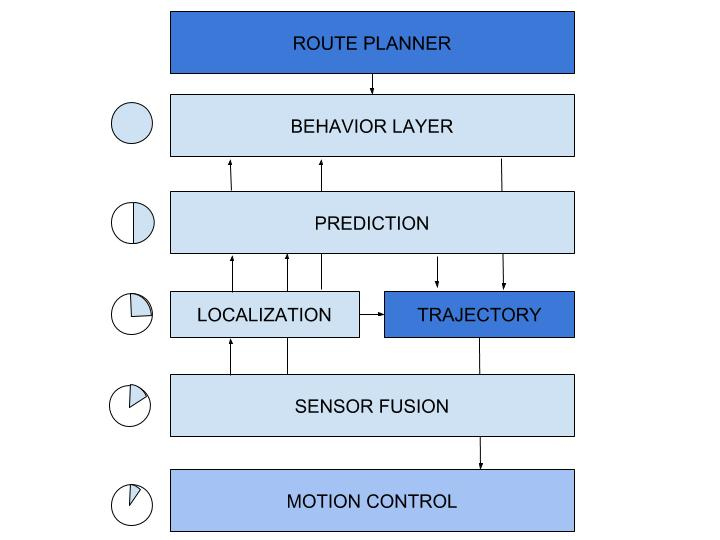
\includegraphics[width=0.8\textwidth]{Images/path_planner.jpg}
    \caption{Path Planning Module}
    \label{path_planner}
\end{figure}

\section{Localization} \label{localization}

Localization module is responsible for providing the current state of the vehicle concerning the position, orientation, speed(linear and angular) and acceleration. The localisation module implemented on the modelcar has two sub-components, Vehicle Odometry and Global Position estimation using Visual GPS. Odometry is calculated with dead reckoning \cite{dead_reckoning} with speed information from motor and Yaw information from Inertial Measurement Unit (IMU). The localisation module combines odometry with the data received from a visual GPS node (tracks markers on the roof) to correctly estimate the state of the ego vehicle. 

\section{Prediction} \label{prediction}

Prediction and Sensor fusion modules receive the data from various sensors such as Cameras, LIDAR, etc. and fuse them together to create an environment model, classifying objects into different categories and predict the state of obstacles in the surroundings. Due to time constraints, this thesis simulates a prediction module to provide motion planner with obstacle information in different traffic scenarios.

\section{Route Planner} \label{route_planner}
Route Planner is responsible for finding a global route between the current vehicle state and the goal state based on the static characteristics of the environment/map such as lane information, speed limits etc. Route planner obtains this information generally from the maps or other formats to represent the road network. In this thesis a simple model called " Road Navigation Definition File (RNDF)"  \cite{rndf_darpa} \cite{rndf_fu} is used to represent the route network. Next subsections details further about RNDF and global reference route calculation.

\subsection{RNDF}

This section details about the RNDF file \cite{rndf_darpa} which defines the road network(set of roads/ areas connected) over which the vehicle can traverse. DARPA developed this representation of road for its Autonomous Vehicles Urban Grand Challenge. RNDF representation first divides the traversable areas into two parts, segments and free zones and provides connections across these areas. Free zones represent areas such as parking lots and road segments represent driving lanes. Each segment has multiple lanes; each lane has waypoints along the driving direction. More significant information about waypoints such as whether it is a stop sign, speed limit, start/end, intersection etc. can be added. Each segment/zone is connected to one another using exits, they represent the connections between one segment waypoints at start/end to another. Figures \ref{rndf_segment} \ref{rndf_exits} \ref{zone_segment} \cite{rndf_darpa} represent different portions of the route representation and Figure \ref{path_Segmentation} details regarding one of the route network of map used in Lab experiments. 


%\begin{figure}
%    \centering
%    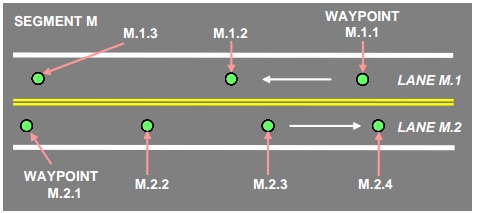
\includegraphics[width=0.6\textwidth]{Images/rndf_segment.png}
%    \caption{Segment representation in RNDF - Segement M has two lanes M1, M2 and each lane has way points 1-N}
%    \label{rndf_segment}
%\end{figure}

%\begin{figure}
%    \centering
%    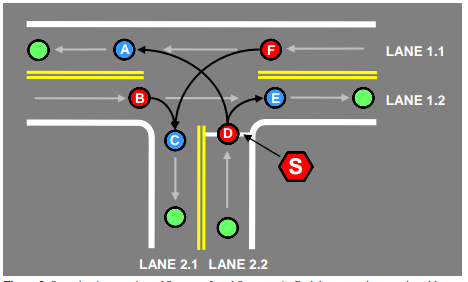
\includegraphics[width=0.5\textwidth]{Images/rndf_exits.png}
%    \caption{Exit representation in RNDF - Connections between two segments in a T-Junction}
%    \label{rndf_exits}
%\end{figure}


\begin{figure}
	\centering
	\begin{subfigure}{.56\textwidth}
	    \centering
		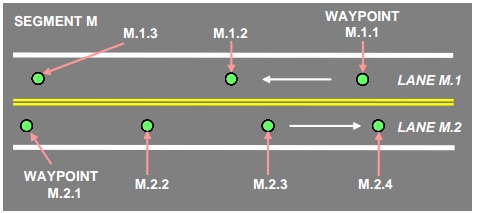
\includegraphics[width=1.0\textwidth]{Images/rndf_segment.png}
		\caption{Segment representation in RNDF - Segement M has two lanes M1, M2 and each lane has way points 1-N}
		\label{rndf_segment}
	\end{subfigure}%
	\begin{subfigure}{.44\textwidth}
		\centering
		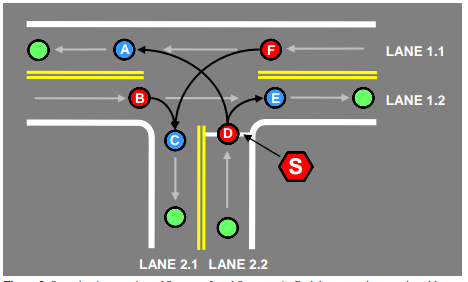
\includegraphics[width=1.0\textwidth]{Images/rndf_exits.png}
		\caption{Exit representation in RNDF - Connections between two segments in a T-Junction}
		\label{rndf_exits}
	\end{subfigure}
	\caption{Path velocity representation in \cite{traj_planner_optimization}}
	\label{rndf_seg_exit}
\end{figure}

\begin{figure}
    \centering
    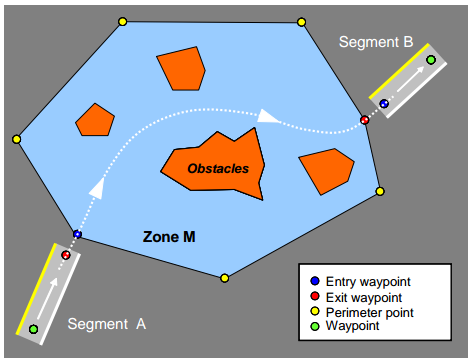
\includegraphics[width=0.5\textwidth]{Images/zone_segment.png}
    \caption{Zone Representation in RNDF - Connection between Segments and Zone}
    \label{zone_segment}
\end{figure}


%\begin{figure}
%    \centering
%    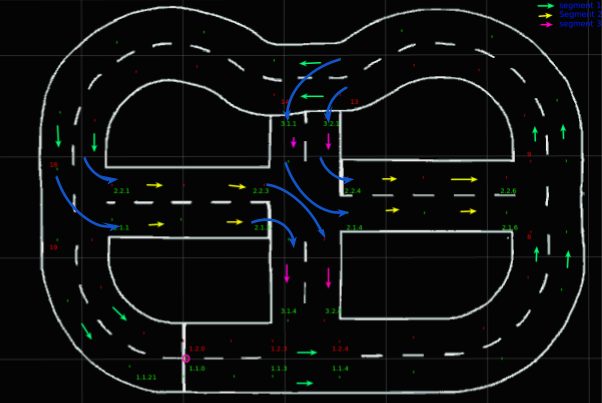
\includegraphics[width=0.8\textwidth]{Images/map_rndf.png}
%    \caption{Road network for the map used to test model Car}
%    \label{map_rndf}
%\end{figure}

\todo{foot note - source of images}
\todo{Add Appendix for how to create the RNDF file for model car}


\subsection{Path Representation and calculation}

The data in RNDF is represented in the form of a tree with connections across way-points. The global path from source to destination is the shortest path between the waypoint closest to the ego vehicle's current position and the waypoint closest to the destination. The shortest path found is subdivided into sub-paths based on the segment to which the waypoints belong. Once the ego vehicle is at the end of one sub-path it receives a notification from the trajectory planner that a goal is reached, then the route planner transmits the next subpath to the trajectory planner, this process is repeated till destination is reached. Figure \ref{path_Segmentation} details further about the division of shortest path across different segments. This method also reduces the memory needed in modelling the road in trajectory planning stage.

\begin{figure}
    \centering
    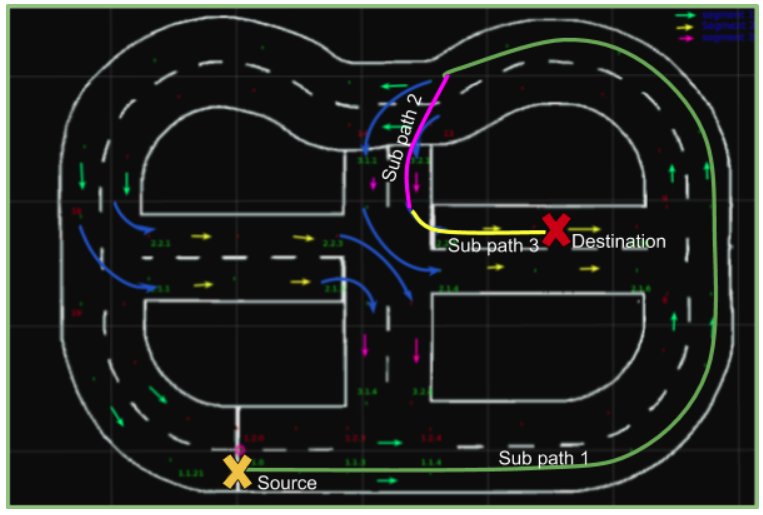
\includegraphics[width=0.8\textwidth]{Images/path_Segmentation.png}
    \caption{Division of shortest path in road network into Sub paths across different segments}
    \label{path_Segmentation}
\end{figure}

\subsection{Behavioral Layer}
\todo{check if this should be moved to related work}
Behavioural layer plays an important role in path planning, it is responsible for understanding the scenario and making decisions according to various traffic rules, constraints and choices that will make driving more efficient for the vehicle. For example, it decides on lane and speed to drive based on constraints such as emptiness of lane, other vehicles in the lane, next needed exit and turn, speed limit etc. The behavioural layer is a huge research topic in itself and not in the scope of this thesis. Currently, a simple simulated approach is implemented where the user can provide inputs to decide behaviour using mouse clicks for lane change and speed information from the map.

\section{Motion Planner} \label{motion_planner}

This section discusses the planning algorithm to create short-term trajectories following the global path to reach the destination. The subsection \ref{timing_constraints} provides an overview of the timing Horizon and constraints in dynamic environments for different modules in planning. The next subsection \ref{frenet_frame} details regarding path modelling and how this will improve the efficiency of planning along with its constraints. It also discusses on approximation method used to convert coordinates from Cartesian to Frenet frame. The core of this section is the creation of trajectories which is discussed in detail in subsection \ref{traj_creation}. The next subsections \ref{osbtacle_check_satic} and \ref{obstacle_check_dynamic} explain further on how the created trajectories are evaluated for collision with static and dynamic obstacles. Next subsection \ref{traj_Selection} details on the selection of final trajectory from the set of evaluated trajectories for the trajectory following.

\subsection{Temporal Horizon} \label{timing_constraints}
Time is an essential aspect of planning in dynamic environments, and there are several timing variables associated with planning. This section is mainly adopted from the doctoral thesis \cite{eth_timing_constraints}. These timing parameters define how far into the future different sub-modules of planning will be valid. 
 \todo{ check if this name is needed and add footnote to link "Autonomous vehicle navigation in dynamic urban environments for increased traffic safety" of Macek kristijan doctoral work} 

The first timing variable in motion planning is timing horizon $ T_m $. It is the measure of how far into the future trajectory of the ego vehicle is planned. Second is the prediction horizon $ T_p $, it is the measure of how far into the future the motion of dynamic obstacles around the ego vehicle can be predicted. The fundamental requirement of planning to be valid is that $ T_m  \le  T_p $ such that planning is done only so far into the future as the environment is predictable. 

Third is $ T_d $, which indicates the computation time of the motion plan. Assuming planning is done in cycles, the plan created in the previous cycle is executed in the current cycle, thus $ T_d  \le  T_m $. If this condition fails, then the planner will run out of path for the next cycle. In general $ T_d \ll T_m $. The fourth timing variable $ T_s $ is the perception update cycle time, i.e., perception module updates the state of surrounding dynamic obstacles every $ T_s $ seconds. In general world, the predicted trajectories for duration $ T_p $ will not hold true, as the behaviour of these vehicles is not controlled by the ego vehicle. Thus the constraint $ T_s  \le T_p $ should be valid. This creates an uncertainty in modelling of the environment. Thus the execution duration of current plan $ T_e $ beyond $ T_s $ is not sensible, this is because obstacle trajectories may have changed in $ T_s $ and executing the old trajectory may lead to collisions invalidating the trajectory created for $ T_m $. 

The next timing constraint in consideration is $ T_e $, control execution time of the current plan. $ T_e $ should not exceed the perception update time $ T_s $. This restriction also imposes additional constraint on $ T_d $ (motion plan computation time), $ T_d \le T_e $. 

In summary, timing constraints described above identify the relation between different modules such as motion planning, motion prediction and execution. It is also important to predict farther into future than $T_s$ or $T_e$ for completeness of motion planner concerning goal objective. In general a farsighted uncertain motion plan potentially directing the vehicle towards goal is better, but this plan needs to be re-evaluated and re-executed in short intervals for correctness. 

\todo{check if this should be moved to implementation}
In general behaviour of obstacles and participants can be predicted for up-to 5s probabilistically. Thus the temporal $ T_m $ \& prediction $ T_p $ horizon are chosen to be 5s. The planner has an execution time $ T_d $ far less than 100ms on a low power computational hardware which allows a high update rate allowing lower values for $ T_e $. As obstacle detection is simulated a pessimistic value of 250ms for $ T_s $ is chosen, and even higher update frequency can be chosen as the planner is fast enough to react. 

\todo{time to see minimum distance ahead with current speed, minimum time to bring car to halt at good speed etc etc. }

\subsection{Path Modelling} \label{frenet_frame}

 The planned global path is in the Cartesian coordinate system. One of the problems with the Cartesian coordinate system is that the due to variation in curvature of the road, local planning becomes complex. To address this issue planning in curvilinear system or Frenet Frame or  lane adoptive (SL) coordinate system has been adopted by researchers, \cite{traj_planner_optimization} \cite{spatio_temporal_state_lattice} \cite{diss_shui_phd_thesis} \cite{real_time_traj_plan_article} \cite{volvo_reactive_traj} \cite{curvilinear_System_Automated_Drv} are some of the research works in which Frenet frame is adopted. In this method centre of the lane/road or preplanned global path is used as reference longitudinal coordinate (S) and perpendicular distance with respect to the lane centre is considered as lateral coordinate (L/D) as represented in Figure \ref{sl_over_xy} \cite{diss_shui_phd_thesis}.  Thus once converted, (S, L) coordinate system essentially is a straight road.
 
 \begin{figure}[H]
    \centering
    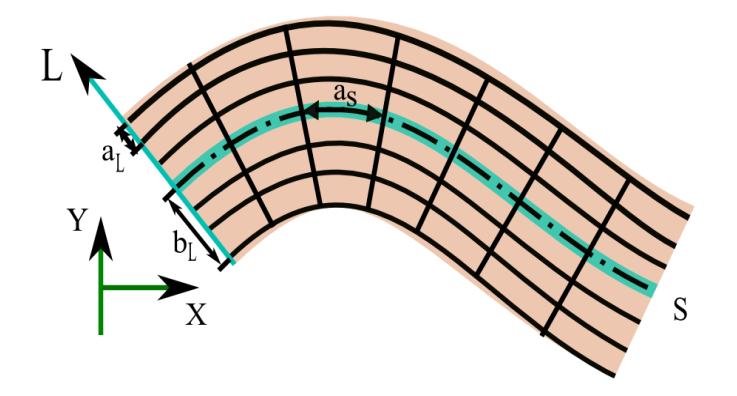
\includegraphics[width=0.8\textwidth]{Images/sl_over_xy.png}
    \caption{SL coordinate system laid over XY coordinate system - \cite{diss_shui_phd_thesis}}
    \label{sl_over_xy}
\end{figure}
 
 Conversion from Frenet frame to Cartesian and vice versa is a widely researched topic and many techniques exist which offer different levels of complexity and accuracy. In this thesis, an approximation method is used to convert between these two coordinate systems similar to \cite{volvo_reactive_traj}. This method is computationally inexpensive and provides a required level of accuracy for the model car. To convert an XY coordinate to SL coordinate, (x,y) is projected onto the current path represented by straight lines joining waypoints as in figure \ref{xy_sl_conversion}, cumulative distance till this point gives the S coordinate, and the perpendicular distance between the projected point and the current point provides the L coordinate. A similar process is used to convert S,L coordinate to x,y coordinate. S is used to find a point on a segment represented by waypoints, a point at a perpendicular distance L gives the x,y coordinate. We assume that the path between two waypoints is linear which reduces the computational complexity in approximation. This approximation, however, approaches zero error when the spacing between two waypoints approaches zero. Adding dense waypoints in the curves significantly reduces the approximation error. There are different methods discussed in \cite{lengthparameterized}, \cite{Wangrobustand} which provide better accuracy in calculating the paths. 

As observed in Figure \ref{sl_over_xy}, in SL coordinate system the size of the unit distance is not constant, it stretches in the convex side of the road and gets compressed in the concave side of the reference line. This is especially an issue in curves with a lower radius of curvature, as it affects velocity planning thus leading to discomfort in some cases. There is extensive research on the topic of velocity and path smoothening which counter these effects. 

In summary, the curvilinear coordinate system makes planning easier but needs extra computation in the conversion from one format to other. It also introduces some errors and inefficiencies in planning if the complete planning is done in SL coordinate system and these need to be addressed. 
 
 \begin{figure}[H]
    \centering
    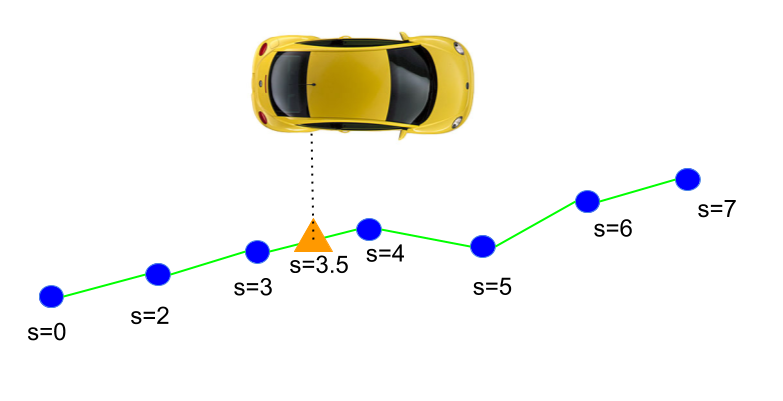
\includegraphics[width=0.8\textwidth]{Images/xy_sl_conversion.png}
    \caption{Showing projection of the current position of the car shown by green triangle to s coordinate system. Each circle represents a node, and the lines between them are links. \cite{volvo_reactive_traj}}
    \label{xy_sl_conversion}
\end{figure}
\todo{add VOLVO reference reference in foot note and also remove the orange dots}


\subsection{ Trajectory Creation} \label{traj_creation}

The core of this thesis is the trajectory planner that drives the robot from source to destination. By understanding the behaviour of human drivers in structured environments (road networks), it is necessary that the trajectory planner creates trajectories that avoid collisions, align with the road network, are smooth, continuous and comfortable. Chapter \ref{related_work} discusses various planning techniques used by different planners. 

%The approach of this thesis to create trajectories is inspired by \cite{unit_A_star} which proposes a trajectory planning technique combining path and velocity planning.

The approach proposed in this thesis is inspired by human driving, i.e., the driver tries to maintain an optimal speed, next shift laterally based on obstacles ahead and brake if a collision is predicted with current driving state or perform an evasive manoeuvre. To reach a speed vehicle need to accelerate/decelerate, this can be achieved with various levels of values based on current state as, each acceleration/deceleration level chosen will result in different final states. The initial step is to sample set of acceleration profiles, Figure \ref{accelerations} shows different acceleration profiles the ego vehicle can follow in time horizon. Currently, constant acceleration profiles are used due to measurement errors in the ego, once state approximation is improved the planner can be switched to trapezoidal acceleration profiles as shown in sub-figure\ref{accelerations}. A1 represents an acceleration of around $2m^{-2}$ and A8 of up to $-8m^{-2}$ which is on the higher end of decelerations, most of the cars are not capable of achieving such large decelerations because of various factors such as road condition, tires etc. Generally deceleration values are up to $-4.5m^{-2}$ \cite{denmark_breaking} \cite{accelerations_study} \cite{accelerations_study_2}. Applying each of this acceleration profile to current ego vehicle state for planning horizon $ T_m $ leads to different final states of ego vehicle. The final sates will have different final velocity as shown in Figure \ref{velocities}, different distances traversed as in Figure \ref{distances}.

Change of acceleration is defined as jerk and to create smooth trajectories it is important that the trajectories generated by the motion planner must have least jerk. There are various techniques to create these jerk free trajectories as discussed in chapter \ref{related_work}. The selection of smoothness also depends on the capabilities of the ego vehicle and controller to track these fine trajectories.
 
 \begin{figure}
    \centering
    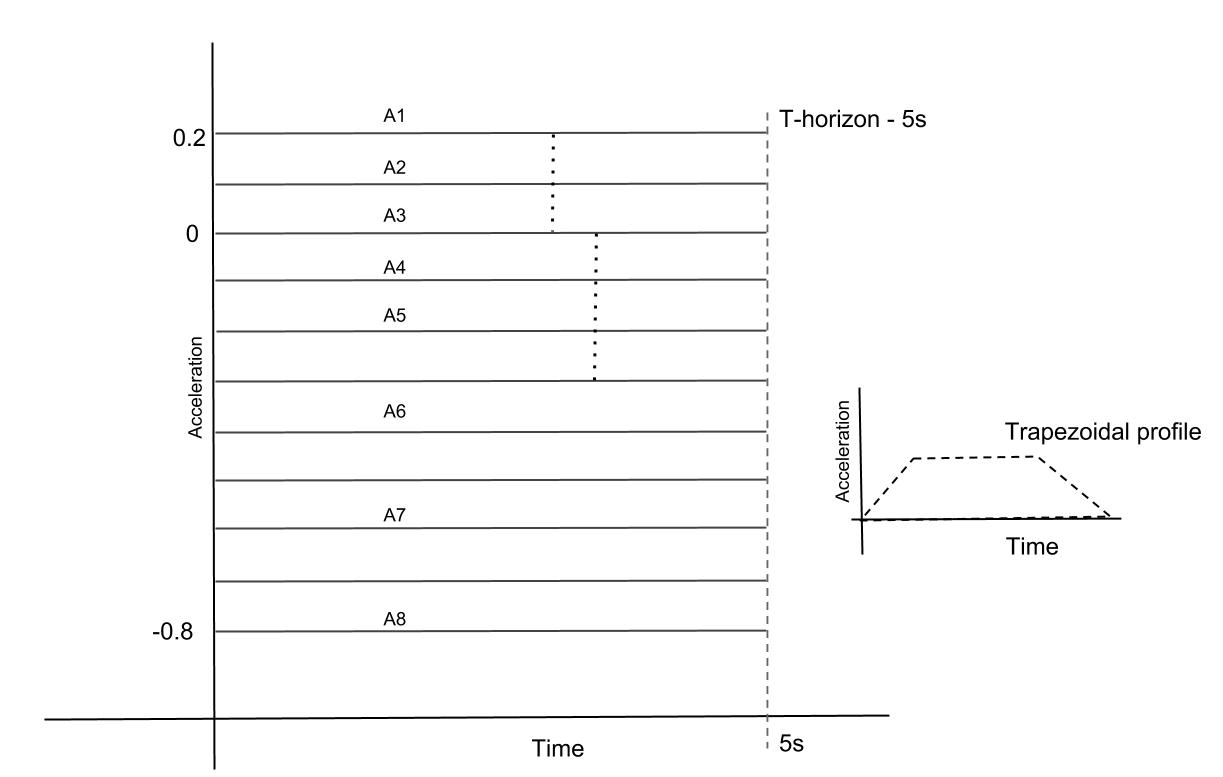
\includegraphics[width=0.8\textwidth]{Images/accelerations2.jpg}
    \caption{Different acceleration profiles a car can follow from current state.}
    \label{accelerations}
\end{figure}

 \begin{figure}
    \centering
    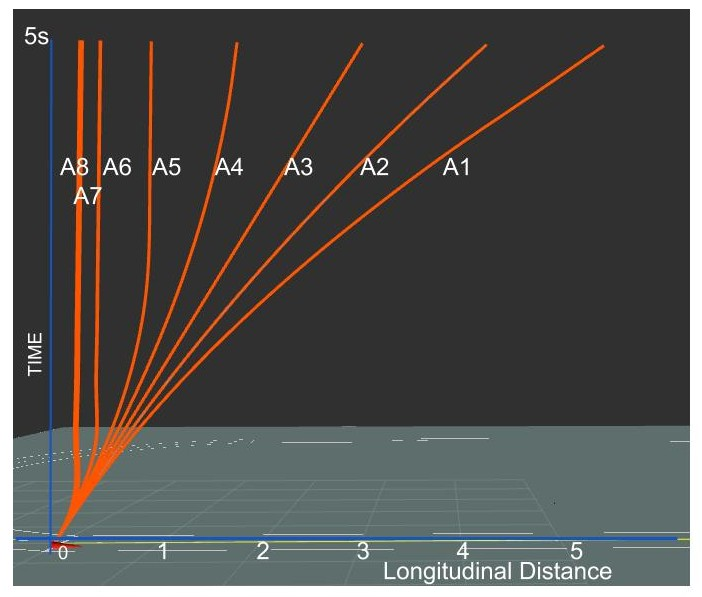
\includegraphics[width=0.8\textwidth]{Images/concept/distvstime2.jpg}
    \caption{Distance traversed vs time with accelerations A1-A8 from \ref{accelerations} in time horizon(5s), Initial position = (0,0) velocity = 0.6$ms^{-1}$, target velocity = 1.5 \& 0 $ms^{-1}$}
    \label{distances}
\end{figure}

 \begin{figure}
	\centering
	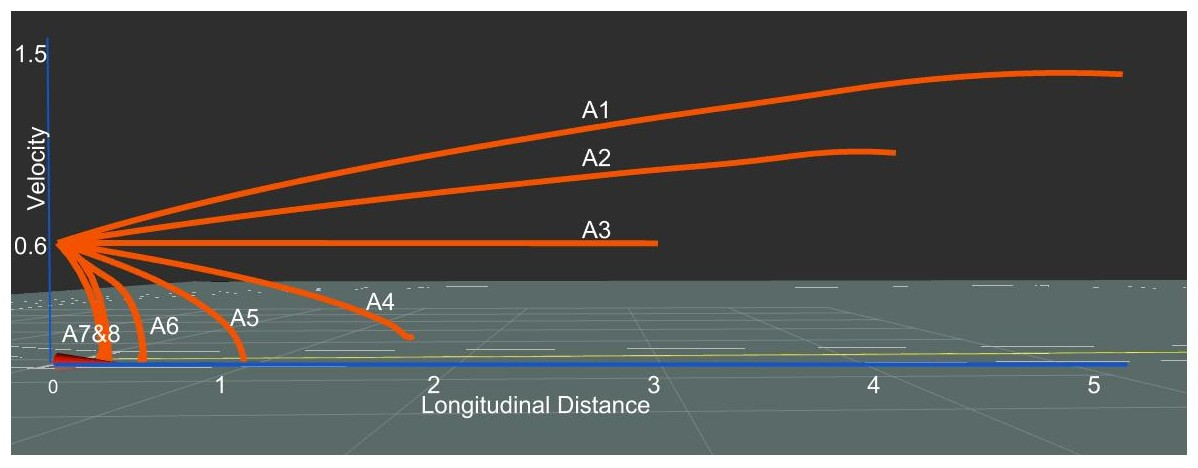
\includegraphics[width=0.8\textwidth]{Images/concept/distvsvel2.jpg}
	\caption{Distance traversed vs Velocity achieved with accelerations A1-A8 from \ref{accelerations} in time horizon(5s), Initial position = (0,0) velocity = 0.6$ms^{-1}$, target velocity = 1.5 \& 0 $ms^{-1}$}
	\label{velocities}
\end{figure}


Acceleration profiles discussed previously solve the problem of longitudinal planning but to avoid obstacles the ego vehicle should also plan lateral (sideways) shifts in its trajectory. Similar to different accelerations, lateral shifts are sampled and combined along with acceleration samples to create final states. Lateral shifts can be mapped either as a function of time or distance traversed by ego vehicle. The research of Werling et al. \cite{werling_frenet} suggests that at lower speeds it is advantageous to map lateral shift as a function of distance and at a higher speed as a function of time. As this thesis is intended towards urban environments with limited speeds, lateral shift is mapped as a function of distance traversed. Lateral shift planning in this thesis is adopted from \cite{real_time_traj_plan_article}, which uses cubic splines and models lateral shift as a parameter of longitudinal distance as shown in equation \ref{lat_shift_one}. 

\begin{equation}
l(s) = c_0 + c_1s + c_2s^2 + c_3s^3
\label{lat_shift_one}
\end{equation}

The first and second derivative of the equation \ref{lat_shift_one} are equations for lateral velocity \ref{lat_vel} and acceleration \ref{lat_acc}.

\begin{equation}
    \frac{dl}{ds} = c_1 + 2c_2s + 3c_3s^2
\label{lat_vel}
\end{equation}


\begin{equation}
    \frac{d^2l}{d^2s} = 2c_2 + 6c_3s.
\label{lat_acc}    
\end{equation}

From the boundary conditions (0- initial state, f - final state), we have

\begin{equation}
l(s_0) = l_0 , l(s_f ) = l_f
\label{lat_boudary}
\end{equation}

The angle between the road frame and the vehicle is defined as $\theta(s)$, it can be derived from the first derivative of the lateral shift with respect to s. 

\begin{equation}
\theta(s) = arctan(\frac{dl}{ds})
\label{lat_veh_theta}
\end{equation}

To ensure the generated path follows current curvature and orientation of car and the final orientation is parallel to the road segment, following conditions should be satisfied.


\begin{equation}
\theta(s_0) = \theta_0 , \theta(s_f) = 0
\label{th_bundary}
\end{equation}

The figure \ref{lat_planning} indicates how the initial orientation will affect the shape of the trajectory. 

 \begin{figure}
    \centering
    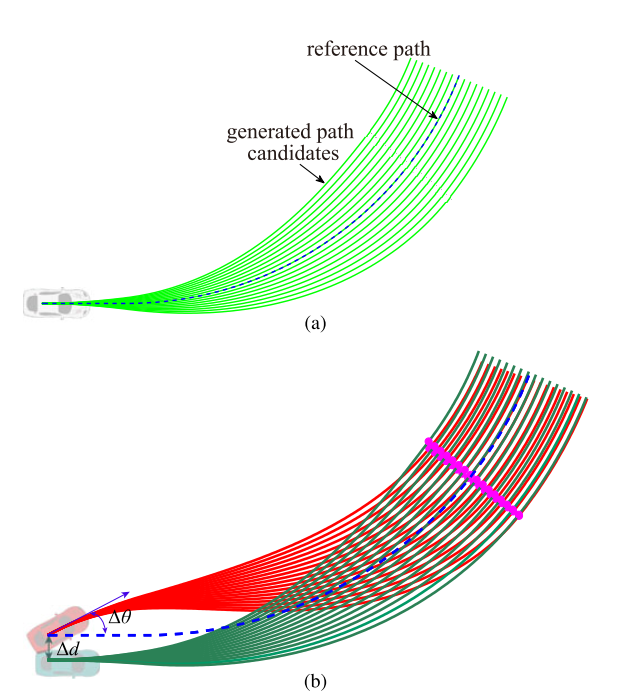
\includegraphics[width=0.8\textwidth]{Images/lateral_planning.png}
    \caption{Path candidates generation results. (a) $l_0 = 0$ and $\theta_0 = 0$ (b) $ 
l_0 = \Delta_d$ and $ \theta_0 = \Delta\theta$. \cite{real_time_traj_plan_article}}
    \label{lat_planning}
\end{figure}

\todo{check if own figure is needed -  remove that sampling terminal states line}


The constants $ { c_0,c_1,c_2,c_3}  $ in equation \ref{lat_shift_one} can be obtained by solving equations \ref{lat_vel} to \ref{th_bundary}.

The Figure \ref{searchspace} represents final search space by ego vehicle in XYT space, the density of this space can be increased by increasing the acceleration profiles and lateral samples. 

 \begin{figure}
	\centering
	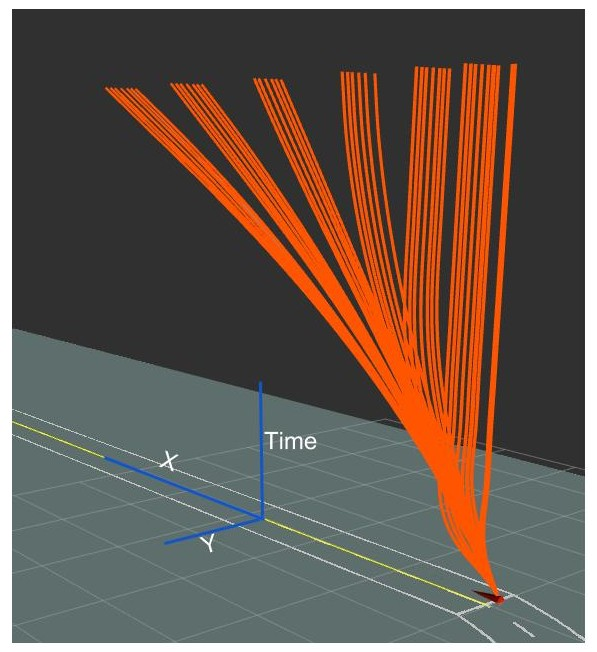
\includegraphics[width=0.8\textwidth]{Images/concept/searchspace2.jpg}
	\caption{Total search space in xyt}
	\label{searchspace}
\end{figure}


\todo{Check if this below suggestion which is not implemented OK to be written here - or mention in implementation due to time constraints}
%Even the short changes in lateral shift create long trajectories that take $T_m$ time, to optimize and increase number of samples, trajectories that traverse lateral shifts in shorter horizon can be added. By ensuring that the samples from last selected trajectory are included in current sample set, smoother and consistent trajectories can be created

In summary, combining samples in acceleration and lateral shifts, multiple trajectories with different final states are created over the time horizon. In the next subsections how these trajectories are tested for collision with respect to static and dynamic obstacles is discussed. 


\subsection{Checking for Static Obstacles} \label{osbtacle_check_satic}
The main objective of the motion planner is to derive a path that is collision free. The generated trajectories must be evaluated for collision or driving close to obstacles. There are various techniques for collision detection as discussed in the background study. This thesis developed a simple two-step collision checking technique for static obstacles. A road parallel model in the Frenet frame is employed for collision checking ignoring the orientation of obstacles with respect to the road as described in \cite{cmu_parallel_thesis}. Using a road parallel method and dilating the obstacle for safety reduces computational complexity. 

\todo{check if all things described in road parallel model for collision checking should be discussed here}

In the first step of collision checking, obstacle coordinates are transformed into Frenet frame and represented by a length and width parallel to the road. In the second step, the trajectory in consideration is checked if it has a collision in longitudinal dimension (S coordinate) for the length of the obstacle. As shown in Figure \ref{static_check} trajectories T0, T1 intersect in S for obstacle O1 and not for obstacle O2. The next step is to find this intersection region, I1 to I2 in Figure \ref{static_check}, the values are dilated for safety. In final it is checked whether from I1 to I2 there is a collision in lateral dimension(d) for trajectory and obstacle. For all points between I1 and I2, the lateral distance between trajectory and obstacle must always be larger than safety value as described in \ref{static_obst_safety_dist}. 

\begin{equation}
    |d\textsubscript{ego} - d\textsubscript{obst}| > car\_width/2 + obstacle\_width/2 + safety\_margin
    \label{static_obst_safety_dist}
\end{equation}
\todo{represent the parameters in terms of $d_e , c_w, o_w$ etc}

It is representative from figure \ref{static_check} that the trajectory T1 has collision and trajectory T0 has no collision. Different costs can be added based on how close the ego vehicle is with respect to the static obstacle. Due to properties of cubic polynomials, it is sufficient to check for the collision at the start, end, middle and min-max D if that falls in the intersected path. 


 \begin{figure}
    \centering
    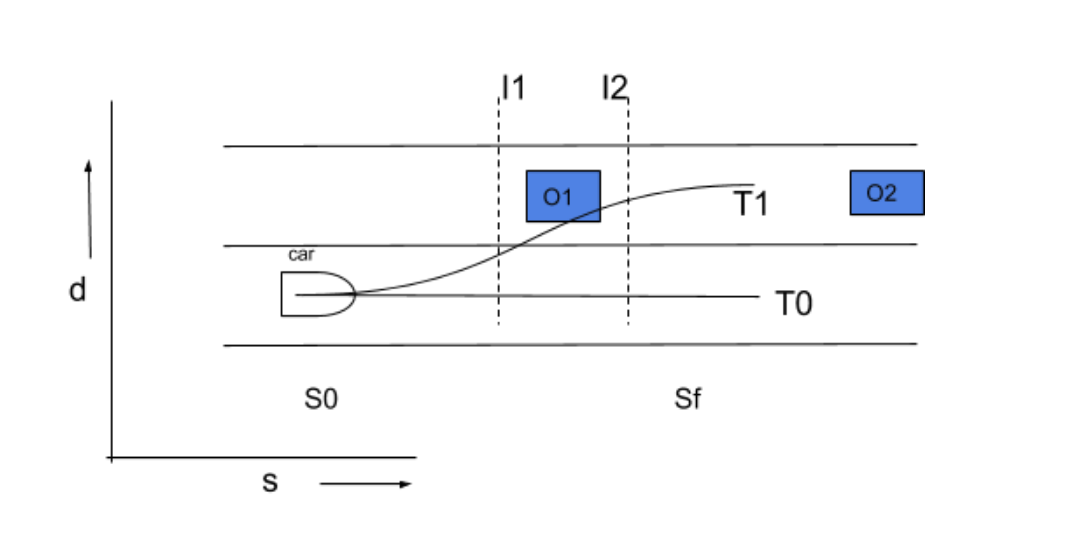
\includegraphics[width=0.8\textwidth]{Images/static_check.png}
    \caption{Collision check for static obstacles}
    \label{static_check}
\end{figure}



\subsection{Checking for Dynamic Obstacles} \label{obstacle_check_dynamic}

In dynamic environments such as cities, it is vital to plan collision-free trajectories by predicting the state of other obstacles. Predicting the future behaviour of obstacles is a challenging part of urban driving, various approaches used are described in subsection \ref{traj_eval}. This thesis models dynamic obstacles as squares continuing with their current speed in their detected lane/lateral position for planning duration similar to \cite{unit_A_star} or moving in opposite direction or moving across the lane based on the angle between the obstacle and road. This assumption can be justified by the fact that the trajectories are re-evaluated at high frequencies and any changes in obstacles lateral distance or orientation will be evaluated in next cycle thus keeping the vehicle safe from the collision. 

The collision check for dynamic obstacles has one extra check-in time dimension as compared to checking for static obstacles, it is inspired by forbidden regions calculation as discussed in \cite{graff_thesis}. In step one the intersection in S coordinate for obstacle and ego vehicle is found, here the length of the obstacle is dilated over the distance travelled by obstacle as represented by dotted line ahead of the obstacle in figure \ref{dynamic_check}. If there is a collision in S dimension, then the collision between ego vehicle and obstacle in lateral dimension (D) in the intersection region I1 to I2 is tested in a similar way to static obstacle collision check. If there is a collision in D dimension, then the corresponding S dimension where there is collision is found, represented with J1-J2 in figure \ref{dynamic_check} (generally this will be shorter than I1 - I2). For the range J1-J2, it is checked if they collide in time also, i.e., if they reach the same location in same time, a buffer time is added to be safe. As per instructions for safe driving it is required for the car to maintain a minimum time gap of 2 seconds with the vehicle ahead. There are more formal methods \cite{mobile_eye_safety_distance} on safety distances for self-driving cars. This thesis implements a simple 2-second rule to safety, and this is a tunable parameter which can be used to increase driving aggression. Figure \ref{dynamic_close1} indicates a similar situation for the collision in time dimension for scenario presented in Figure \ref{dynamic_check} with the difference that the obstacle is in a different lane.

To check collision in time dimension, time difference between the ego vehicle and the obstacle at the S dimension intersection borders is tested as shown in figure \ref{dynamic_time_check}. If the gap is larger than 2 seconds at all the times and doesn't change sign then there is no collision, Figure \ref{dynamic_close1} and \ref{dynamic_close2} present a situation where the time to the collision between ego vehicle and obstacle reduces but there is no collision. If the time difference between ego vehicle and the obstacle has an opposite sign at the start and end of the intersection region, then it detected as a collision. As difference indicates time to collision, and time and distance are continuous a change in sign in time difference demonstrates that in between at some point there was a collision (difference = 0). Figure \ref{dynamic_collision1} and \ref{dynamic_collision2} present a situation where the projected trajectory of the ego vehicle will collide with a dynamic obstacle. Figures \ref{dynamic_opp1} represent a case where the planned trajectory of ego vehicle collides with obstacle moving in opposite direction and Figure \ref{dynamic_opp2} represents where the ego vehicles projected trajectory would not collide the vehicle in reverse lane.

Dynamic obstacle moving laterally across the road are represented as static obstacle occupying the length of the road. Thus, if there is a pedestrian crossing the road, the trajectory is considered to be in the collision if there is a collision in S dimension and there will anyways be a collision in D dimension due to dilation of the pedestrian width to the width of the road and no time dimension is checked. This could, however, be improved by checking the direction of walking and also predicting the time to cross the road to check for collision. 

Collision checking in dynamic environments approximated as the path from start to end with linear velocity, in reality, this is not true, and there will be acceleration and deceleration by ego vehicle. Figure \ref{dynamic_approx} presents scenario where the ego vehicle with $0.1ms^{-1}$ velocity is accelerated at $0.4ms^{-2}$, the corresponding approximated line for 5s if line with uniform velocity of $1.1ms^{-1}$. For this approximation to be safe the time difference between the original path and the approximated line should never be greater than $2s$, the maximum time difference as presented by the black line is $0.8s$. The difference is affected mainly by the acceleration and deceleration values with higher values causing a higher shift. Due to limits on maximum speed, acceleration and minimum speed of zero, the approximation holds good for the 5s horizon. To reduce the safety margin to less than 1s, simply adding checks at every second instead of the start and end are sufficient. 

\todo{Should I write the mathematical proof that this approximation works here or in appendix??} 

\todo{Compared to simulation based methods this method is faster to implement and works for different velocities easily, where to write this? }

 \begin{figure}
    \centering
    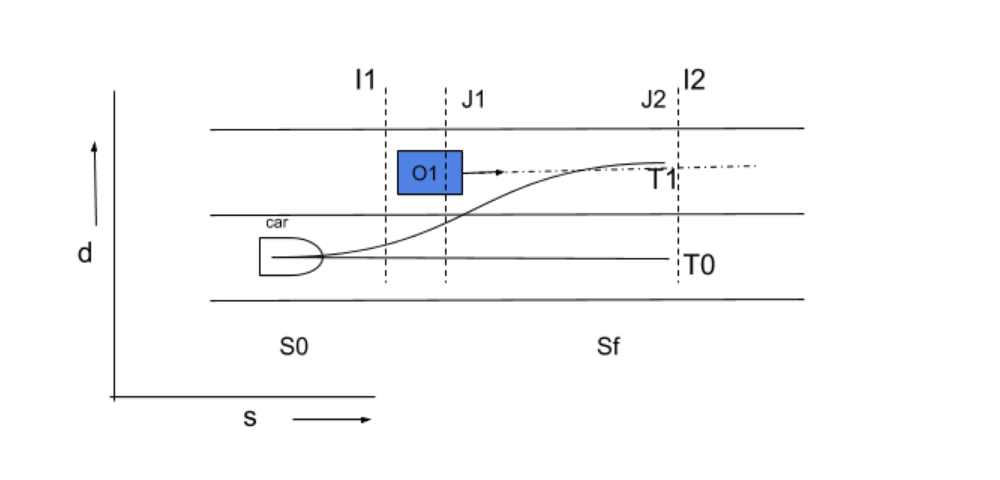
\includegraphics[width=0.8\textwidth]{Images/dynamic_check.png}
    \caption{Collision check for Dynamic obstacles}
    \label{dynamic_check}
\end{figure}

\begin{figure}
	\centering
	\begin{subfigure}{.51\textwidth}
		\centering
		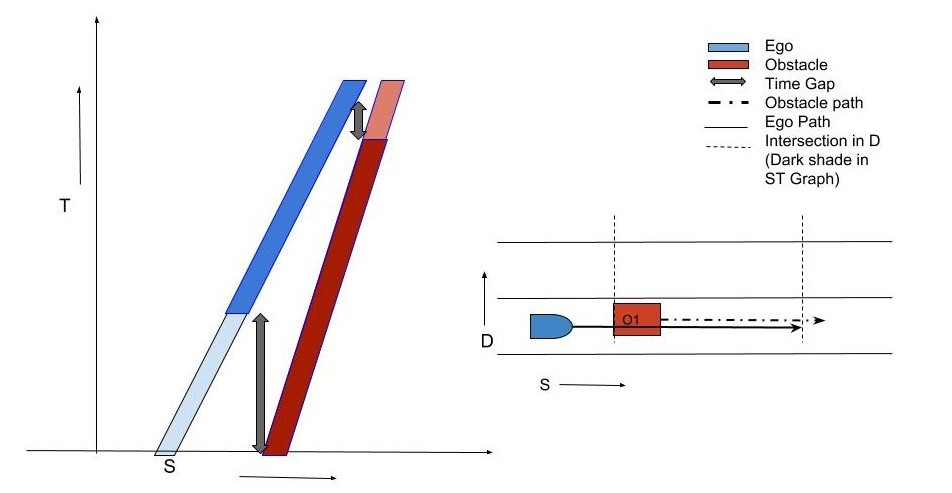
\includegraphics[width=1.0\textwidth]{Images/concept/dynamic_close1.jpg}
		\caption{Ego vehicle projected trajectory getting close to slow moving obstacle ahead}
		\label{dynamic_close1}
	\end{subfigure}%
	\begin{subfigure}{.49\textwidth}
		\centering
		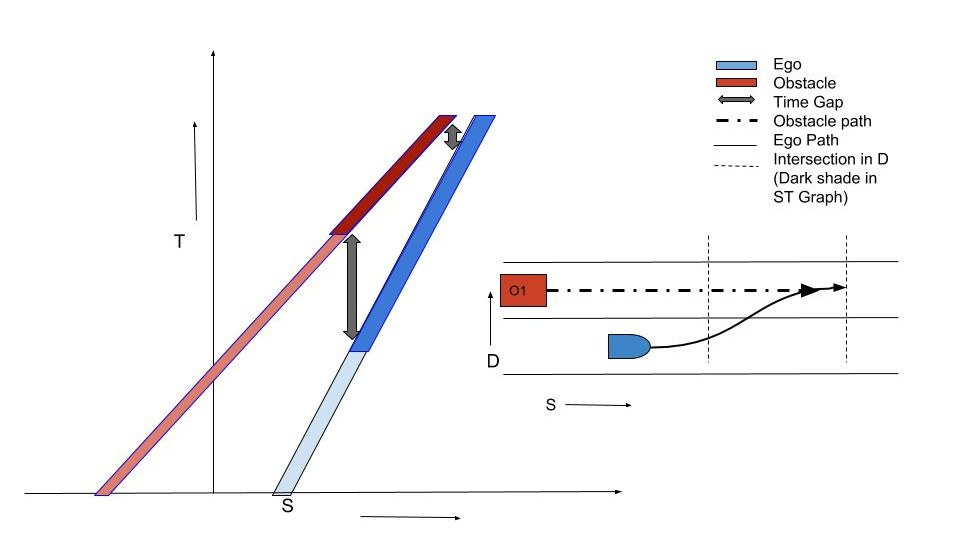
\includegraphics[width=1.0\textwidth]{Images/concept/dynamic_close2.jpg}
		\caption{Ego vehicle projected trajectory getting close to a fast moving dynamic obstacle in next lane while performing a lane change}
		\label{dynamic_close2}
	\end{subfigure}
	\caption{Ego vehicle getting close to dynamic obstacale but not colliding}
	\label{dynamic_close}
\end{figure}


\begin{figure}
	\centering
	\begin{subfigure}{.515\textwidth}
		\centering
		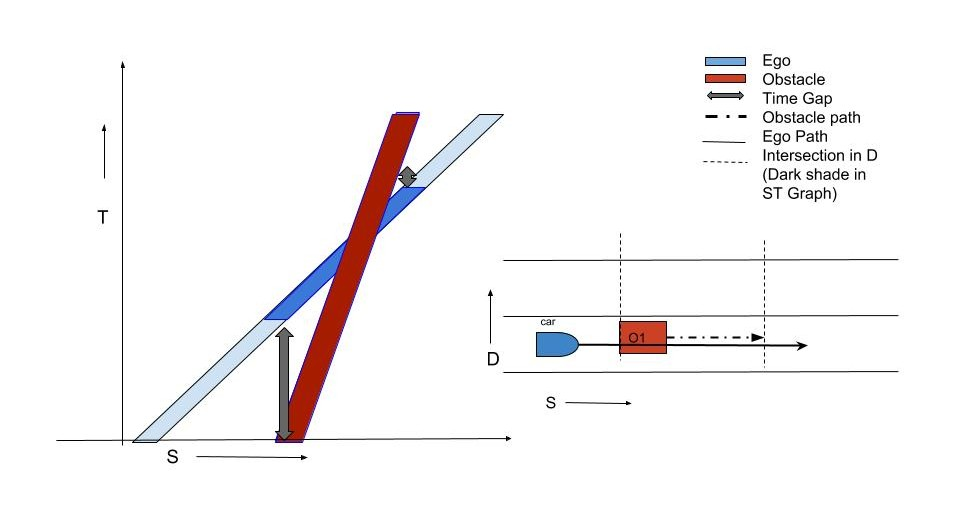
\includegraphics[width=1.0\textwidth]{Images/concept/dynamic_collison.jpg}
		\caption{Ego vehicle projected trajectory colliding with obstacle ahead}
		\label{dynamic_collision1}
	\end{subfigure}%
	\begin{subfigure}{.485\textwidth}
		\centering
		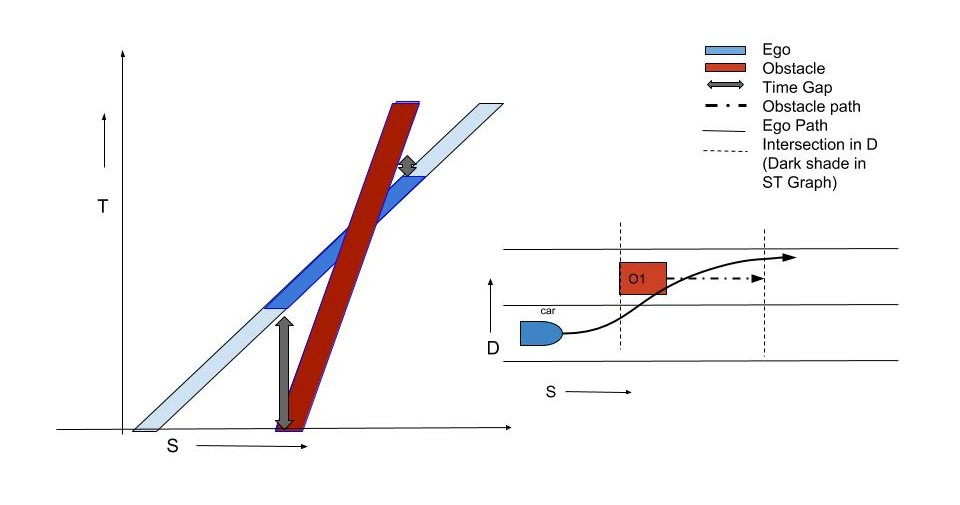
\includegraphics[width=1.0\textwidth]{Images/concept/dynamic_collison2.jpg}
		\caption{Ego vehicle projected trajectory colliding with obstacle ahead while performing lane change}
		\label{dynamic_collision2}
	\end{subfigure}
	\caption{Ego vehicle projected trajectory colliding with obstacle in future.}
	\label{dynamic_collision}
\end{figure}

\begin{figure}
	\centering
	\begin{subfigure}{.515\textwidth}
		\centering
		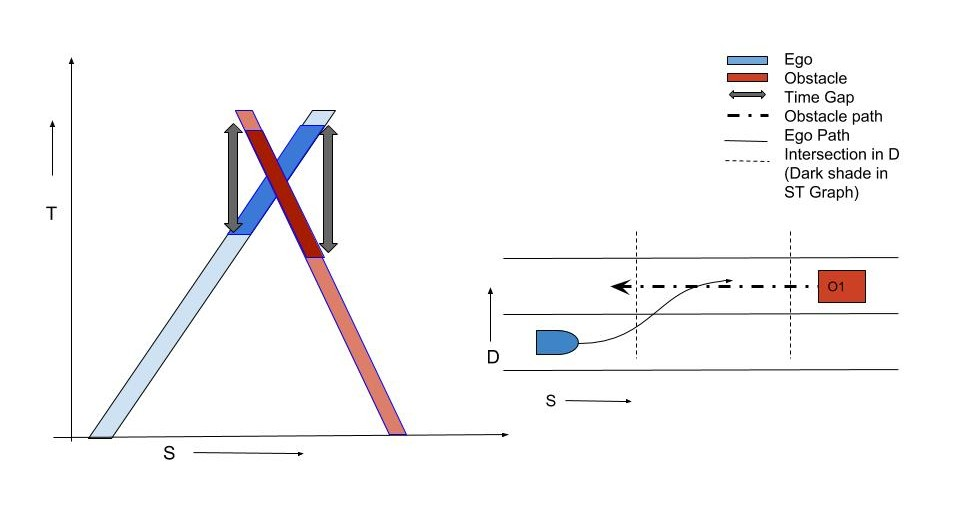
\includegraphics[width=1.0\textwidth]{Images/concept/dynamic_opposite_collision.jpg}
		\caption{Ego vehicle projected trajectory colliding with obstacle moving in opposite direction}
		\label{dynamic_opp1}
	\end{subfigure}%
	\begin{subfigure}{.485\textwidth}
		\centering
		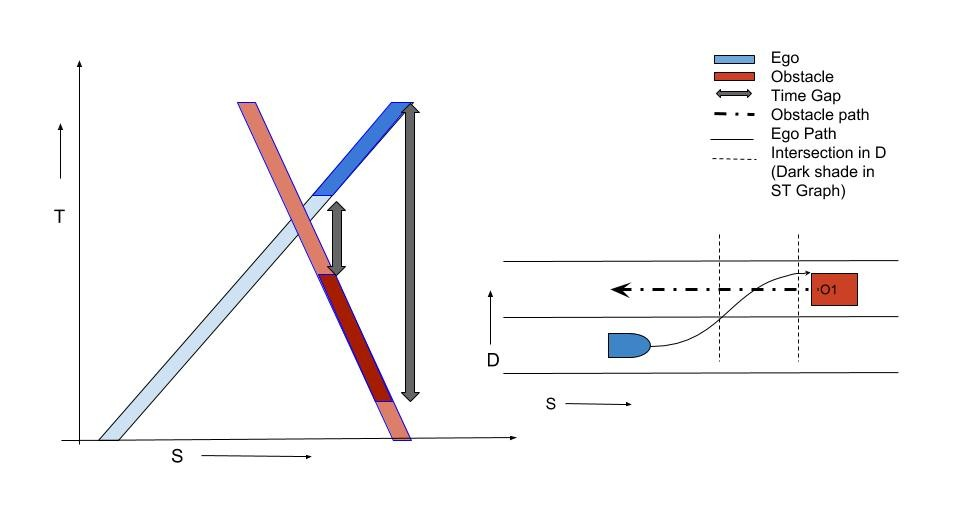
\includegraphics[width=1.0\textwidth]{Images/concept/dynamic_opposite_nocollision.jpg}
		\caption{Ego vehicle projected trajectory performing a lane change and not colliding with obstacle in next lane}
		\label{dynamic_opp2}
	\end{subfigure}
	\caption{Ego vehicles interaction with }
	\label{dynamic_opp}
\end{figure}

 \begin{figure}
	\centering
	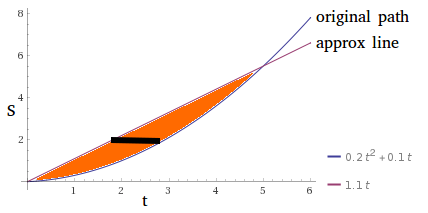
\includegraphics[width=0.8\textwidth]{Images/concept/dynamic_approx.png}
	\caption{Approximation of Parabolic Path to a line}
	\label{dynamic_approx}
\end{figure}

%\begin{figure}
%    \centering
%    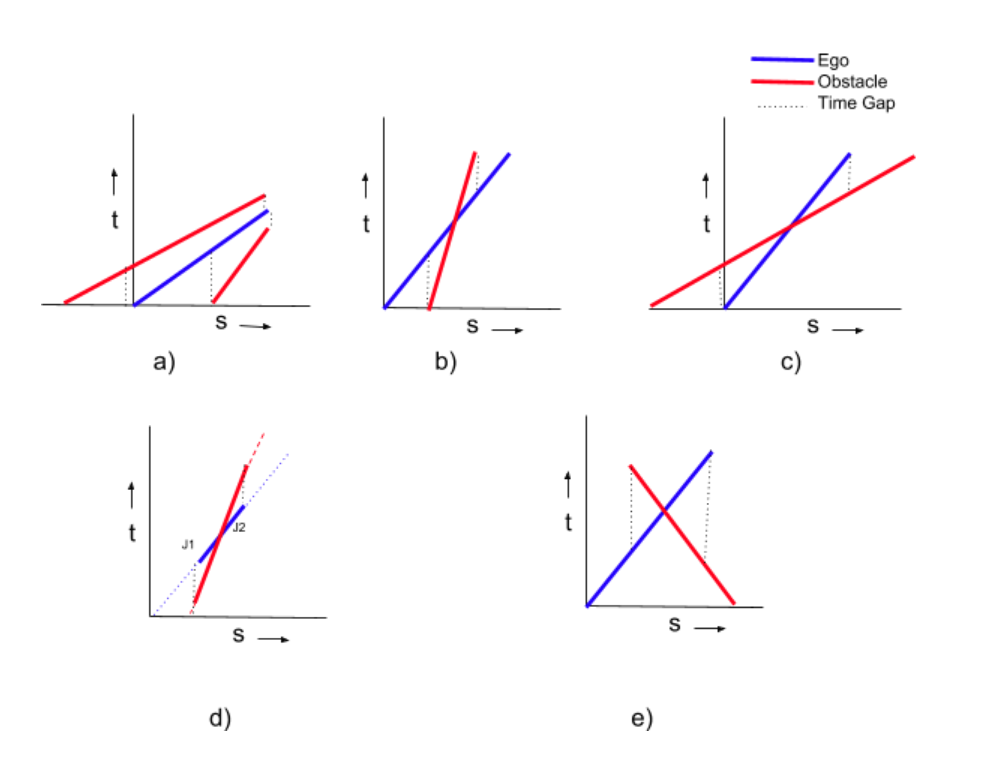
\includegraphics[width=0.8\textwidth]{Images/dynamic_Check_time.png}
%    \caption{Collision check in space Time a) indicates obstacles getting close to the ego vehicle but not colliding. b) Ego vehicle hits the slow moving obstacle ahead. c) Ego vehicle is hit by fast moving obstacle behind - Situation during unchecked lane change by ego vehicle }
%    \label{dynamic_time_check}
%\end{figure}



%Dynamic obstacles are assumed to continue in the lane they are detected and if an obstacle is found across two lanes then it is assumed to be performing lane change and modelled as two dynamic obstacles moving straight in both lanes to overcome uncertainty.


%The collision check dynamic obstacles is performed in two stages, in first stages bounding boxes are drawn across the length of the trajectory of both the ego vehicle and the dynamic obstacle across time T. If the bounding boxes intersect then the second stage of collision check is invoked. In this step, both the dynamic obstacle and ego vehicle are moved in unit steps of time and checked for collision. As per the earlier assumption, dynamic obstacles tend to move in the lane they are detected thus to make the collision check simple, 3 lines are drawn across the corners and centre of the vehicle. The lines are extended for unit time and if the 3 lines intersect with the ego vehicle bounding square then there is a collision. The figure \ref{dynamic_obstacle} details further about the collision check.
%\todo{(The representation is not correct in figure, take the representation from the cited pages for further ease)}
%\todo{bounding boxes - Autonomous Driving in Dynamic Environments}
%\todo{Cite this paper for $3$ line collision-  An RRT-based Navigation Approach for Mobile Robots and Automated Vehicles-RRT*\_. pdf}




\subsection{Cost Functions and Trajectory Selection} \label{traj_Selection}
Selection of final trajectory is based on the different costs associated with it, and costs can be static and dynamic. Static costs are known before trajectory creation and dynamic costs are known after the trajectory is created and evaluated. There is wide research on different costs involved in trajectory selection as discussed in section \todo{add link to subchapter costs in related works}

This thesis implements a simple cost function as represented in \ref{cost_eqn}; explicit smoothness costs are not considered as the target validation platform is a model car with no humans inside and limitations of the model car to track a fine trajectory. 
\begin{equation}
cost = |V_a - V_t| + |a_t| + | (d_t - d_e)*k1 | + | (d_p - d_e)*k2 |\
\label{cost_eqn}
\end{equation}
$V_a$ - velocity achieved by trajectory.
$V_t$ - Target Velocity.
$a_t$ - Target Acceleration.
$d_t$ - Target lateral distance.
$d_e$ - Trajectory lateral distance.
$d_p$ - Previous target lateral for trajectory.
$k_1,k_2$ - Factors to adjust weights, currently used at 0.8 and 0.2

The velocity and acceleration terms in cost function \ref{cost_eqn} promote higher accelerations if the target and current velocity difference are higher and lower accelerations if the difference is low. The next lateral terms promote the trajectories that are closer to the target lateral distance and also close to the previous selection thus limiting the shifts in path selection and maintaining continuity. 

Initially, all the sampled trajectories are assigned the costs based on the cost function \ref{cost_eqn} and sorted, then the trajectory with the lowest cost is evaluated for collisions first. The list is sorted again and evaluated till the top of the list has the lowest cost, and the trajectory is evaluated. 

\subsection{Velocity Planning}
Velocity planning is an important aspect of the planer, in general, behavioural layer defines the target velocity based on speed regulation, other traffic participants, required behaviour, road condition etc. In this thesis, a simple approach of velocity limiting is used based on road curvature to limit lateral accelerations. Max velocity  V\textsubscript{max} is calculated based on the equation \ref{max_vel}. 

\begin{equation}
    V\textsubscript{max} = min(\sqrt{Acc\textsubscript{MaxLat} / |k(s)|} , V\textsubscript{limit})
\label{max_vel}
\end{equation}
$V\textsubscript{limit}$ - Velocity limit mentioned in road network,
$Acc\textsubscript{MaxLat}$ - Maximum Lateral acceleration(based on comfort and vehicle dynamics),
$k(s)$ - Road curvature.

\section{Trajectory Follower} \label{traj_follower}

Check whether to refer to MIG trajectory controller or write in short about the controller. 
